\lstset{
  basicstyle=\ttfamily\small,
  breaklines=true,                 
  breakatwhitespace=true,          
  frame=lines,                     % Changed from 'single' to 'lines' for elegant page breaking
  framesep=0.5em,
  backgroundcolor=\color{gray!10},
  keywordstyle=\color{blue}\bfseries,
  commentstyle=\color{gray}\itshape,
  stringstyle=\color{red},
  showstringspaces=false,
  captionpos=t,                    % Locks the caption to the top of the listing
  abovecaptionskip=0.5em,
  belowcaptionskip=0.5em,
  aboveskip=1.5em,                 % Adds breathing room above the listing
  belowskip=1.5em                  % Adds breathing room below the listing
}

\chapter{Design and Implementation}\label{chap:chapter5}

\section{Knowledge Base Design}

\hl{Implemented in the architectural design is a structured knowledge base that stores scenarios, user profiles, and their corresponding conversation logs. The knowledge base is designed to support personalization of advice and feedback by maintaining a comprehensive record of user metrics and interactions. The database schema includes the following:}

\begin{itemize}
    \item \hl{\textbf{User Profiles} - Contains user information, primarily withholding personally identifiable information and pragmatic competence metrics (Intention Coherence, Social Nuance, and Communicative Effectiveness) that are updated after each conversation session.}
    \item \hl{\textbf{Conversation Logs} - Contains the transcripts of conversations corresponding to each user, along with the associated pragmatic analysis scores and feedback generated by the AI Mentor.}
    \item \hl{\textbf{Scenarios} - Contains a collection of predefined conversational scenarios, each with its own context, goals, and dialogue data that the AI Partner uses for role-playing during conversations.}
\end{itemize}

\hl{These tables are designed to be relational for querying and are primarily hosted in Supabase. The user profiles and conversation logs are linked via a foreign key relationship, as illustrated in Tables \ref{tab:user_profiles}, \ref{tab:conversation_logs}, and \ref{tab:scenarios_json}, while the scenarios are an independent JSON file loaded into the system.}

\begin{table}[h!]
\centering
\caption{User Profiles Table Schema}
\label{tab:user_profiles}
\begin{tabular}{p{4cm} p{2.5cm} p{8cm}}
\hline
\textbf{Column Name} & \textbf{Data Type} & \textbf{Description} \\ \hline
\texttt{user\_id} & UUID (PK) & Unique identifier issued by Supabase Auth. \\
\texttt{username} & String & The user's display name or parsed email prefix. \\
\texttt{sessions\_completed} & Integer & Cumulative count of finished conversation scenarios. \\
\texttt{avg\_intention\_coherence} & Float & Running average score (0.0 to 1.0) for Intention. \\
\texttt{avg\_social\_nuance} & Float & Running average score (0.0 to 1.0) for Social Nuance. \\
\texttt{avg\_communicative\_eff} & Float & Running average score (0.0 to 1.0) for Effectiveness. \\
\texttt{holistic\_greeting\_cache} & JSONB & Stores the most recent mentor greeting to reduce API calls. \\
\texttt{holistic\_mentor\_history} & JSONB & Persisted history of the user's Q\&A with the Holistic Mentor. \\ \hline
\end{tabular}
\end{table}

\begin{table}[h!]
\centering
\caption{Conversation Logs Table Schema}
\label{tab:conversation_logs}
\begin{tabular}{p{3.5cm} p{2.5cm} p{8.5cm}}
\hline
\textbf{Column Name} & \textbf{Data Type} & \textbf{Description} \\ \hline
\texttt{id} & Integer (PK) & Auto-incrementing unique identifier for the session log. \\
\texttt{user\_id} & UUID (FK) & Foreign key linking the log to the specific user profile. \\
\texttt{scenario\_id} & Integer & The ID of the scenario the user practiced. \\
\texttt{transcript} & Text & The raw, line-by-line chat history of the session. \\
\texttt{feedback\_text} & Text & The formatted Markdown feedback report generated by the AI. \\
\texttt{session\_scores} & JSONB & The raw JSON object containing the 8 pragmatic sub-scores. \\
\texttt{mentor\_chat\_history} & JSONB & Post-session Q\&A dialogue querying the specific feedback. \\
\texttt{session\_timestamp} & Timestamp & UTC timestamp of when the session was completed. \\ \hline
\end{tabular}
\end{table}

\begin{table}[h!]
\centering
\caption{Scenarios JSON Schema Structure}
\label{tab:scenarios_json}
\begin{tabular}{p{3.5cm} p{2.5cm} p{8.5cm}}
\hline
\textbf{Key} & \textbf{Data Type} & \textbf{Description} \\ \hline
\texttt{id} & Integer & Unique identifier for the scenario. \\
\texttt{title} & String & User-facing title of the scenario (e.g., "The Pauwi Na Curfew"). \\
\texttt{thematic\_conflict} & String & The developmental theme mapping to Arnett and Havighurst. \\
\texttt{chatbot\_role} & String & The persona the AI Partner must adopt. \\
\texttt{opening\_line} & String & The exact first message the AI Partner sends to initiate chat. \\
\texttt{full\_description} & String & The system prompt instructions injected into the AI Partner. \\ \hline
\end{tabular}
\end{table}

\hl{The tables are populated with no initial data except for the scenarios table, which contains a pre-populated and pre-defined set of conversational scenarios curated by the researchers. The user profiles and conversation logs are populated as users interact with the system. The user profiles are created upon registration and the conversation logs are created after each conversation session. Moreover, the user profile metrics are updated after each conversation session based on the pragmatic analysis by the AI Mentor, with the metrics averaged over the course of multiple conversation sessions to track the user's progress over time. These updates are accomplished by the Flask backend, which receives the accumulating information and conversation data after each session and writes it to the database accordingly.}


\section{Software Design and Implementation}

\hl{The chatbot system is built on top of a large language model, namely Gemini 3 Flash via the google-genai SDK, implemented using Python with a Flask server backend, and follows a dual-agent system architecture consisting of the AI Partner and the AI Mentor.}

\hl{In this architecture, the system orchestrates multiple instances of \texttt{gemini-3-flash-preview}, each configured with specific Thinking Budgets and system instructions to balance real-time latency with deep pragmatic analysis.}

\subsection{Agent Instances and Configuration}
\hl{To achieve nuanced pedagogical feedback, the system utilizes four distinct configurations of Gemini 3 Flash:}

\begin{itemize}
    \item \hl{\textbf{AI Partner (Roleplay)} This instance is configured with a lower thinking budget (512 tokens) and prioritizes fast response times for fluid conversation.}
    \item \hl{\textbf{AI Mentor (Pragmatic Analysis)} This instance is configured with a higher thinking budget (8000 tokens) to allow for computationally heavy analysis of user responses. It utilizes a JSON schema containing the 3 categories and its 8 subcategories for the mapping of quantitative scoring.}
    \item \hl{\textbf{AI Mentor (Post-session Feedback)} This instance operates with a medium thinking budget (1,500 tokens) for generating in-session feedback based on the analysis from the Pragmatic Analysis instance.}
    \item \hl{\textbf{Holistic Mentor} This instance is configured with a higher thinking budget (8000 tokens) similar to the pragmatic analysis instance. This agent focuses on aggregating user data and conversation logs to provide holistic and personalized feedback}
\end{itemize}

\subsection{System Workflow}
\begin{itemize}
    \item \hl{\textbf{DOM Load} - The Document Object Model (DOM) loads the user interface built on HTML, CSS, and Flask (Python).}
    \item \hl{\textbf{Profile Initialization} – The system authenticates the user and initializes their profile, loading quantitative metrics and historical data.}
    \item \hl{\textbf{Holistic Analysis} - The Holistic Mentor analyzes longitudinal metrics and user data to recommend a scenario suited to the user's current needs.}
    \item \hl{\textbf{Scenario Selection} - After the user elects to create a new chat, the system loads the scenarios list on the UI, allowing the user to select a scenario to converse in.}
    \item \hl{\textbf{Load Dialogue Data} - Once the scenario is selected, the system loads the corresponding dialogue data and formats the interface to reflect the scenario's context and goals.}
    \item \hl{\textbf{System Prompts} - The system loads the system prompts for the AI Partner, focused on roleplaying the selected scenario.}
    \item \hl{\textbf{Interact via Conversation Engine} – The user engages in real-time dialogue with the AI Partner.}
    \item \hl{\textbf{Conversation End} - Once the user ends the conversation, the system saves the conversation to the database and aligns the conversation data to the user's profile.}
    \item \hl{\textbf{Pragmatic Analysis} - The AI Mentor analyzes the conversation data using the quantitative scoring framework (Intention Coherence, Social \& Affective Nuance, and Communicative Effectiveness) and provides the user with feedback on their performance and areas for improvement.}
    \item \hl{\textbf{In-depth Feedback} - The user may then ask follow-up questions to gain further insight into their performance by continuing to speak to the AI Mentor, which takes into consideration the full conversation data.}
\end{itemize}

\begin{figure}[H]
    \centering
    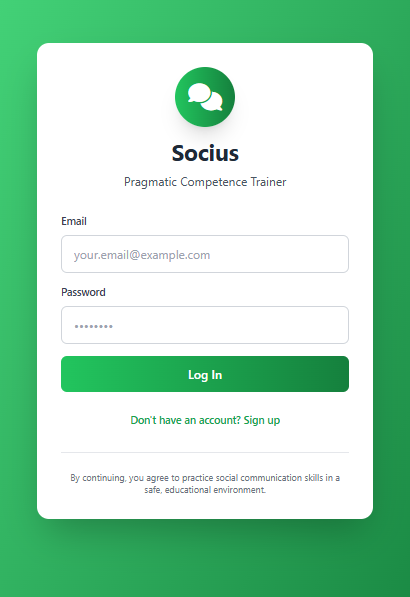
\includegraphics[width=0.85\textwidth]{figures/authentication_screen.png}
    \caption{Authentication Screen}
    \label{fig:authentication_screen}
\end{figure}

\hl{As shown in Figure \ref{fig:authentication_screen}, the authentication screen and profile initialization allow users to sign in and have their profile data loaded. This accomplishes personalization of the system, as the user's historical data and metrics are now available for the system to utilize --- particularly for the Holistic Mentor's ability to recommend scenarios based on the user's current needs, and for the user's ability to request in-depth feedback regarding their complete conversational history. The profile also allows the user to view their progress over time across multiple conversations through the metric dashboard, shown in Figure \ref{fig:holistic_analysis_dashboard}, while the user's overall pragmatic competence summary is accessible via the Profile Screen shown in Figure \ref{fig:profile_screen}.}

\begin{figure}[H]
    \centering
    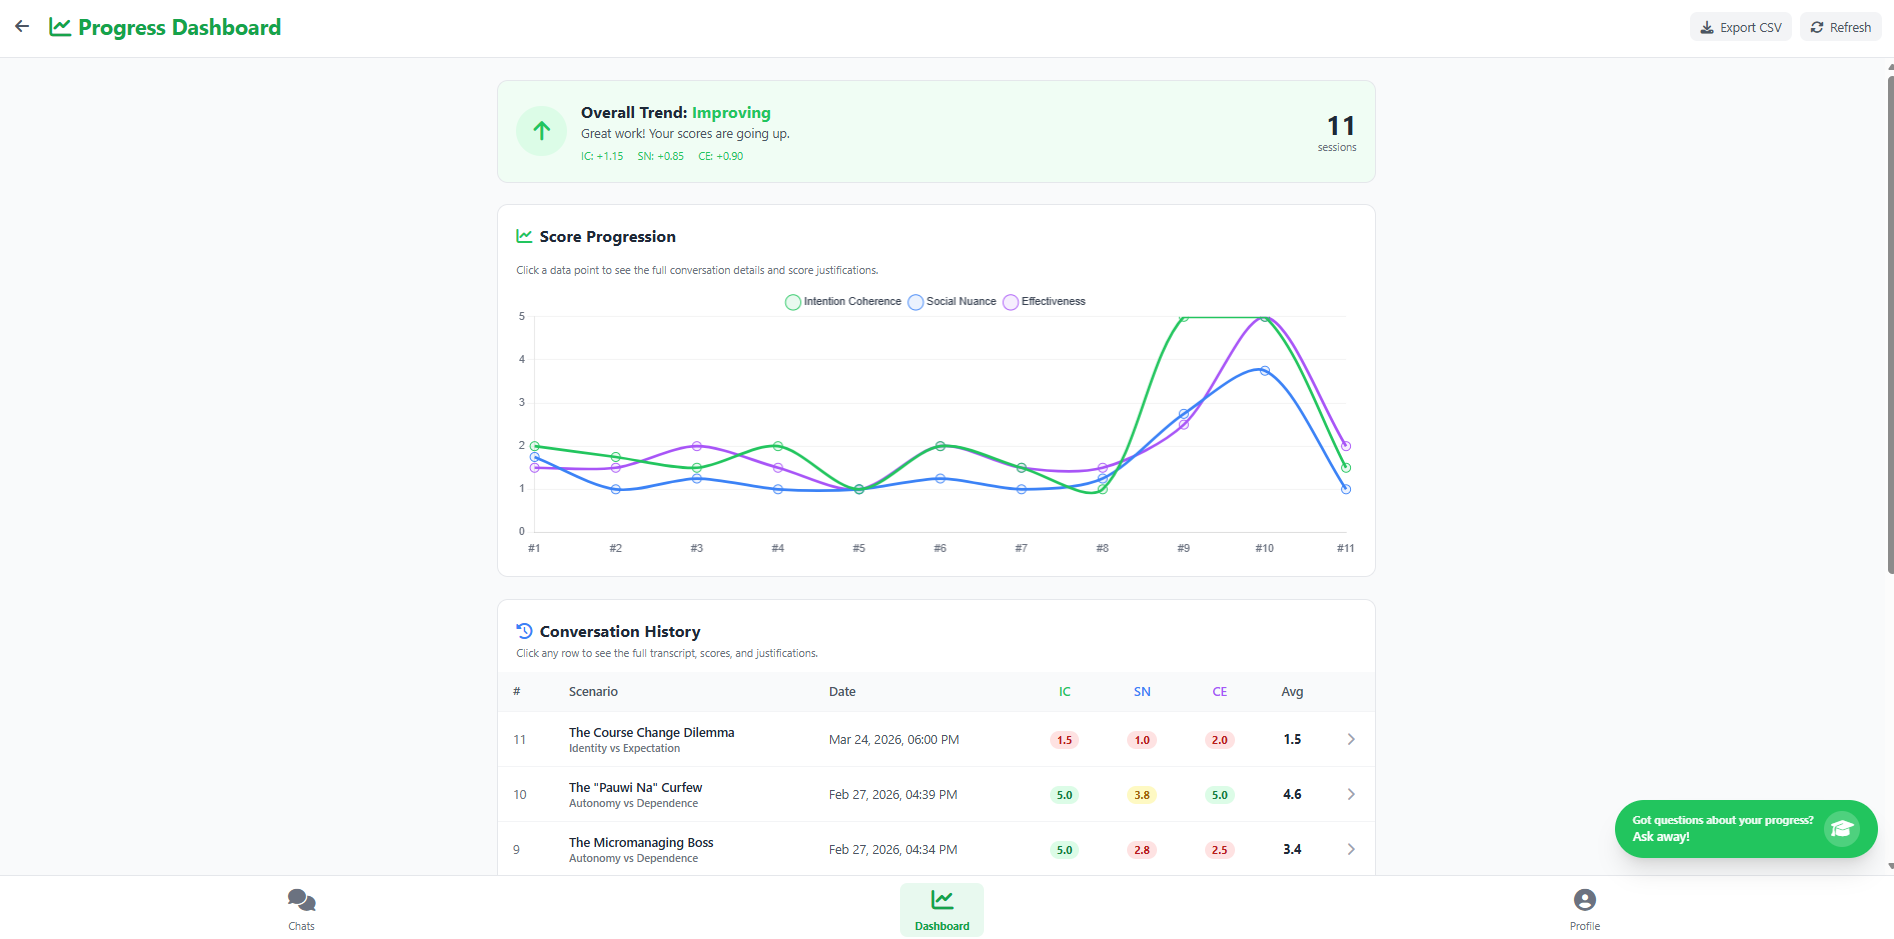
\includegraphics[width=0.85\textwidth]{figures/progress_dashboard.png}
    \caption{Holistic Analysis and Dashboard Screen}
    \label{fig:holistic_analysis_dashboard}
\end{figure}

\begin{figure}[H]
    \centering
    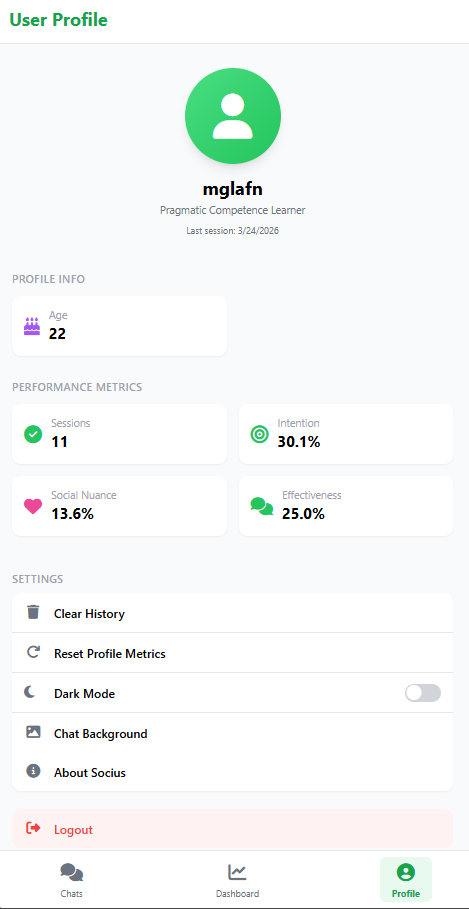
\includegraphics[width=0.85\textwidth]{figures/profile_screen.png}
    \caption{Profile Screen}
    \label{fig:profile_screen}
\end{figure}


\hl{Firstly, the DOM loads with the Flask server, then user data is received for authentication and profile initialization. This allows the system to personalize the experience based on the user's history, metrics, and overall profile and pragmatic competence.}

\hl{The Holistic Mentor then analyzes the user's pragmatic scores and profile to recommend a scenario suited to their current needs. Once the user selects the button to create a new chat, the scenarios list loads on the UI, allowing the user to select a scenario. Once the scenario is selected, the system loads the corresponding dialogue data and formats the interface to reflect the scenario's context and goals, then loads the system prompts for the AI Partner focused on roleplaying the scenario.}

\hl{The user then engages in a back-and-forth conversation with the AI Partner, which employs system prompts focused on responding in a human-like manner while considering the social environment and the persona it is roleplaying. Once the user ends the conversation, the system saves the conversation to the database and aligns the conversation data to the user's profile.}

\hl{The conversation is then analyzed by the AI Mentor using the quantitative scoring framework (Intention Coherence, Social \& Affective Nuance, and Communicative Effectiveness), which provides the user with feedback on their performance and guidance for improvement in future conversations. The user may then click a button to gain further insight into their performance by continuing to speak to the AI Mentor, which takes into consideration the full conversation data.}

\subsection{Scenario Selection and Dialogue Loading}
 
\hl{The scenario selection subsystem is the entry point of every practice session. It is implemented as a two-phase process coordinated between the Flask backend and the client-side JavaScript in \textit{index.html}.}
 
\hl{In the first phase, when a user opens the new-chat modal, the browser issues a \textit{GET} request to the \textit{/api/scenarios} Flask endpoint, which calls \textit{load\_scenarios()} from \textit{src/utils.py}. This function reads the \textit{data/scenarios.json} file into memory and returns the full catalogue of eleven pre-authored scenarios to the client. The catalogue is organized around four thematic conflicts drawn directly from the theoretical framework: \textit{Identity vs. Expectation}, \textit{Autonomy vs. Dependence}, \textit{Ambiguity vs. Definition}, and \textit{Group vs. Self}. Each scenario object in the JSON file carries the following fields: a unique integer \textit{id}, a \textit{title}, a \textit{thematic\_conflict} tag, a \textit{chatbot\_role} description for the AI Partner, a short \textit{opening\_line} that the AI Partner delivers verbatim at the start of the conversation, and a \textit{full\_description} string containing the complete scene-setting context injected into the AI Partner's system instruction. The client renders these records as selectable cards in the scenario selection modal, grouped by thematic conflict so that the user can identify which developmental challenge each scenario addresses.}
 
\hl{In the second phase, once the user selects a scenario as shown in Figure \ref{fig:scenario_selection_modal}, the client sends a \textit{POST} request to the \textit{/api/start-session} endpoint, passing the chosen \textit{scenario\_id} and the authenticated \textit{user\_id}. The backend then: (1) fetches the matching scenario object from the in-memory catalogue; (2) instantiates a fresh \textit{SociusChatbot} object; (3) calls \textit{chatbot.set\_scenario(chosen\_scenario['full\_description'])}, which appends the scenario's full context to the base \textit{AI\_PARTNER\_SYSTEM\_INSTRUCTION} and re-creates the partner's chat session with this updated system instruction; and (4) calls \textit{chatbot.inject\_opening\_line(opening\_line)}, which inserts the partner's first utterance directly into the SDK's internal chat history so that it appears as an authentic model-turn rather than a synthetic user prompt. The session is then stored in the server-side \textit{chatbot\_sessions} dictionary under a randomly generated \textit{session\_id}, alongside the chosen scenario object, the \textit{user\_id}, and a creation timestamp used for TTL-based cleanup. The response payload returns the \textit{session\_id}, the full scenario object, and the \textit{opening\_message} string, which the client immediately displays as the first message bubble in the conversation window.}
 
\begin{figure}[H]
    \centering
    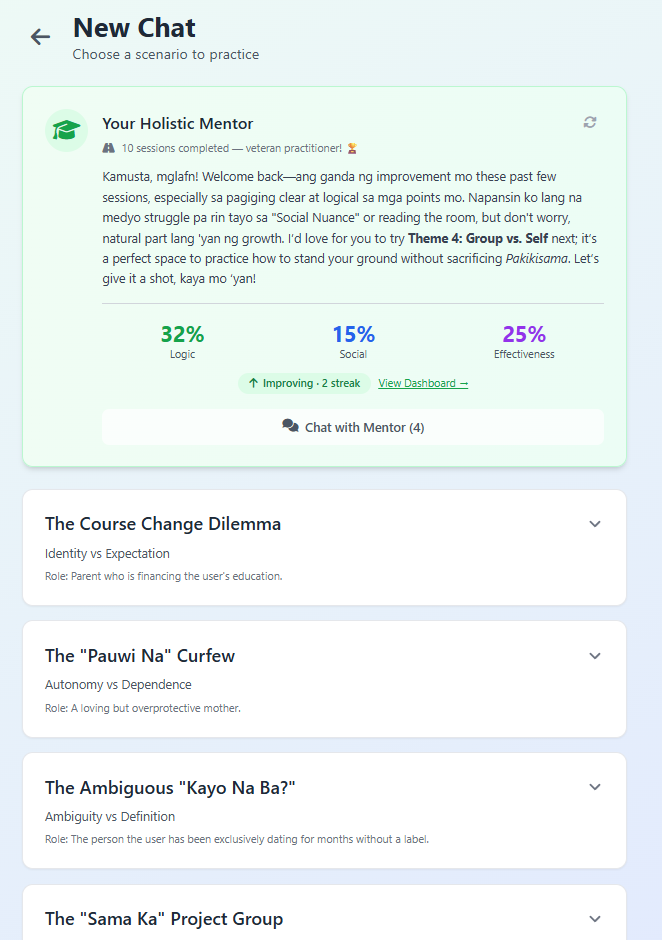
\includegraphics[width=0.85\textwidth]{figures/actual_newchat_arrow_ui.png}
    \caption{Scenario Selection Modal}
    \label{fig:scenario_selection_modal}
\end{figure}

\subsection{AI Partner and Real-Time Conversation Flow}
 
\hl{The AI Partner is the conversational agent with which the user directly interacts during a practice session. It is implemented as a persistent chat session managed by the \textit{SociusChatbot} class in \textit{src/chatbot.py}, using the \textit{google.genai} SDK's stateful \textit{chats.create()} interface. This approach preserves the full multi-turn dialogue history natively within the SDK object, removing the need for the application to manually reconstruct conversation context on every API call.}
 
\hl{The AI Partner instance is configured with three deliberate choices that reflect the system's pedagogical design. First, a thinking budget of 512 tokens (\textit{thinking\_level = "low"}) is assigned via the \textit{ThinkingConfig} object. This allows the model to perform lightweight chain-of-thought reasoning which is sufficient for cue-reading and character consistency, while keeping latency low enough for real-time conversation. Second, the model's temperature is set to 1.0 to encourage naturalistic variation in dialogue, preventing responses from feeling robotic or repetitive. Third, the \textit{AI\_PARTNER\_SYSTEM\_INSTRUCTION} encodes specific rules for generating authentic Taglish speech, including prohibitions against parenthetical English translations, mandates for Filipino conversational markers (\textit{diba}, \textit{kasi}, \textit{naman}, \textit{nga}), and context-sensitive formality rules - formal characters such as bosses or professors are explicitly instructed to suppress casual Taglish fillers, while familial or peer characters are encouraged to use them freely.}
 
\hl{Message delivery is implemented using Server-Sent Events (SSE) via the \textit{/api/stream-message} endpoint, producing the conversation interface shown in Figure \ref{fig:conversation_screen}. When the user submits a message, the client issues a \textit{POST} request and the Flask backend opens an event-stream response that calls \textit{chatbot.stream\_partner\_response(user\_input)}. This generator function invokes \textit{chat\_session.send\_message\_stream()}, iterates over the response chunks as they arrive from the Gemini API, and yields each chunk as a JSON-encoded SSE frame of the form \textit{data: \{"chunk": "text"\}}. The client receives and progressively appends these chunks to the partner's message bubble, creating a real-time typewriter effect. A terminal \textit{\{"done": True, "role": "chatbot\_role"\}} frame signals completion. A quota-aware retry wrapper, \textit{\_try\_stream\_with\_rotation()}, monitors for rate-limit exceptions and transparently backs off before retrying, making sure the session remains stable under API pressure.}
 
\begin{figure}[H]
    \centering
    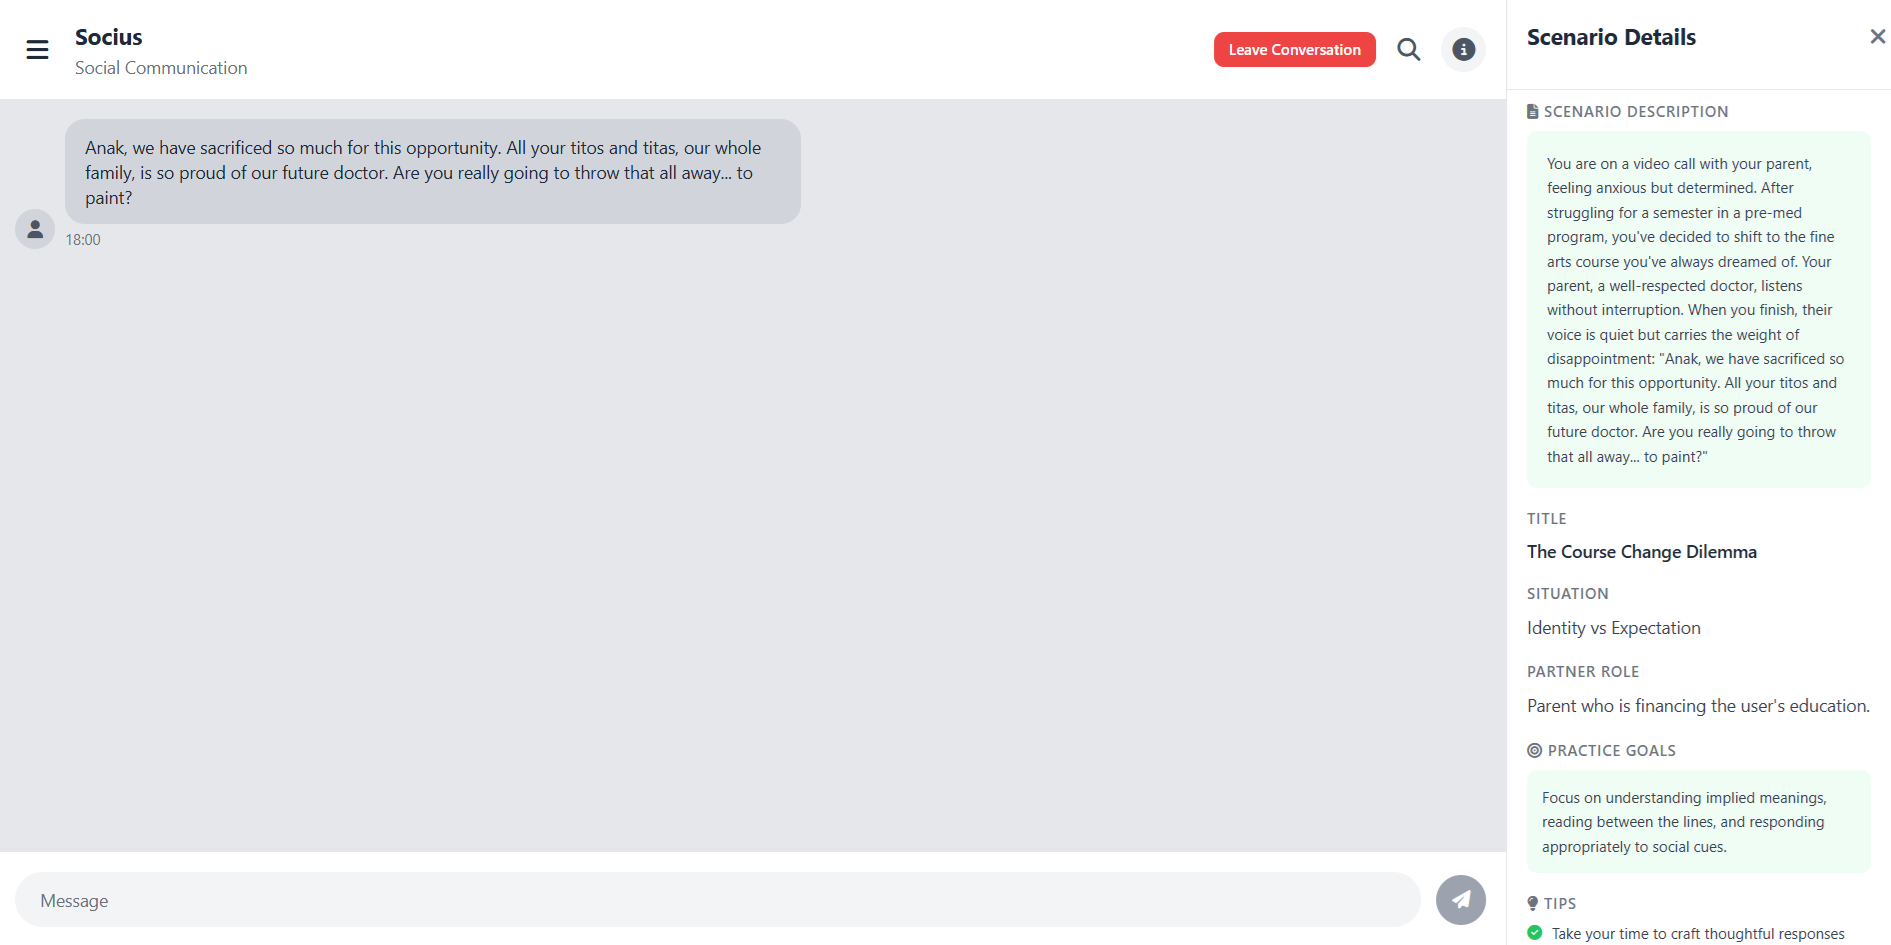
\includegraphics[width=0.85\textwidth]{figures/actual_chat_ui.png}
    \caption{Active Conversation Screen - real-time streaming of AI Partner responses}
    \label{fig:conversation_screen}
\end{figure}
 
\hl{The conversation loop continues until the user clicks the ``End Session'' button, at which point the client posts to \textit{/api/end-session} and the application transitions to the post-session analysis phase. As a fault-tolerance mechanism, the client maintains a local copy of the full message history throughout the session. Should the server-side session expire before the user ends the conversation (the TTL is 30 minutes), the client supplies this local transcript in the \textit{/api/end-session} payload, enabling a stateless recovery path in the backend that reconstructs the scenario context from the \textit{scenario\_id} and runs the pragmatic analysis on the client-supplied transcript directly, without requiring an active \textit{SociusChatbot} session.}

\subsection{Pragmatic Logging and Post-Session Analysis}
 
\hl{Upon session termination, the system executes a two-stage routine that transforms the raw conversation transcript into structured pedagogical data and persists it to the database.}
 
\hl{\textbf{Stage 1: Combined Analysis (Single API Call).} The pragmatic analysis is performed by a dedicated \textit{gemini-3-flash-preview} instance configured with a thinking budget of 8,000 tokens (\textit{thinking\_level = "high"}) and a structured JSON output schema enforced through Gemini's \textit{response\_mime\_type = "application/json"} and \textit{response\_schema} parameters. The analysis is triggered by \textit{chatbot.end\_session\_and\_analyze()}, which calls the internal \textit{\_run\_pragmatic\_analyzer()} method. This method extracts the full conversation transcript from the SDK's curated chat history, appends a system end-tag, and constructs the Combined Analysis Prompt Template by interpolating the scenario context and the transcript. The prompt instructs the model to produce both quantitative scores and qualitative feedback in a single generation pass, reducing API overhead compared to a two-call approach.}
 
\hl{The output is constrained to the \textit{SCORING\_RESPONSE\_SCHEMA}, a JSON schema defining two top-level objects. The \textit{pragmatic\_scores} object contains three category nodes: \textit{intention\_coherence}, \textit{social\_affective\_nuance}, and \textit{communicative\_effectiveness}. They are each with a floating-point \textit{score} on a 1--5 scale, a \textit{sub\_scores} object containing granular metrics, and a string \textit{justification} citing specific transcript evidence. Specifically, Intention Coherence resolves to two sub-scores: \textit{Speech Act Clarity} and \textit{Discourse Flow}. Social \& Affective Nuance resolves to four sub-scores: \textit{Formality Level}, \textit{Emotional Empathy}, \textit{Informativeness}, and \textit{Cultural Filipino Values}. Communicative Effectiveness resolves to two sub-scores: \textit{Implicature Handling} and \textit{Goal/Persuasion Achievement}. The top-level \textit{score} for each category is the arithmetic mean of its sub-scores. The \textit{feedback} object carries five string fields: \textit{key\_takeaway}, \textit{cooperative\_efficiency}, \textit{relational\_management}, \textit{conversational\_achievement}, and \textit{actionable\_tip}. Because the output is enforced as valid JSON via Gemini's native schema constraint, the backend parses the response with a single \textit{json.loads()} call without any additional defensive processing.}
 
\hl{\textbf{Stage 2: Database Persistence.} After analysis, the Flask backend writes two records to Supabase. First, a new row is inserted into the \textit{conversation\_logs} table via \textit{profile.add\_conversation\_log()}, storing the \textit{user\_id}, \textit{scenario\_id}, the plaintext transcript, the formatted \textit{feedback\_text} string, the complete \textit{session\_scores} JSON object, and a UTC timestamp. Second, the user's running average scores in the \textit{user\_profiles} table are updated via \textit{profile.update\_pragmatic\_profile()}, which converts each raw 1--5 score to a 0.0--1.0 decimal using the formula $\frac{score - 1}{4}$ and recalculates the cumulative running average:}
 
\[
\bar{x}_{n} = \frac{\bar{x}_{n-1} \times (n-1) + x_n}{n}
\]
 
\hl{where $\bar{x}_{n-1}$ is the previous running average, $n-1$ is the count of previously completed sessions, and $x_n$ is the new session's normalized score. This formula is applied independently to all three competency dimensions and the result is rounded to four decimal places before being written back to Supabase. The updated profile metrics then become available to the Holistic Mentor for subsequent sessions. The resulting feedback report presented to the user is shown in Figure \ref{fig:post_session_feedback}.}
 
\begin{figure}[H]
    \centering
    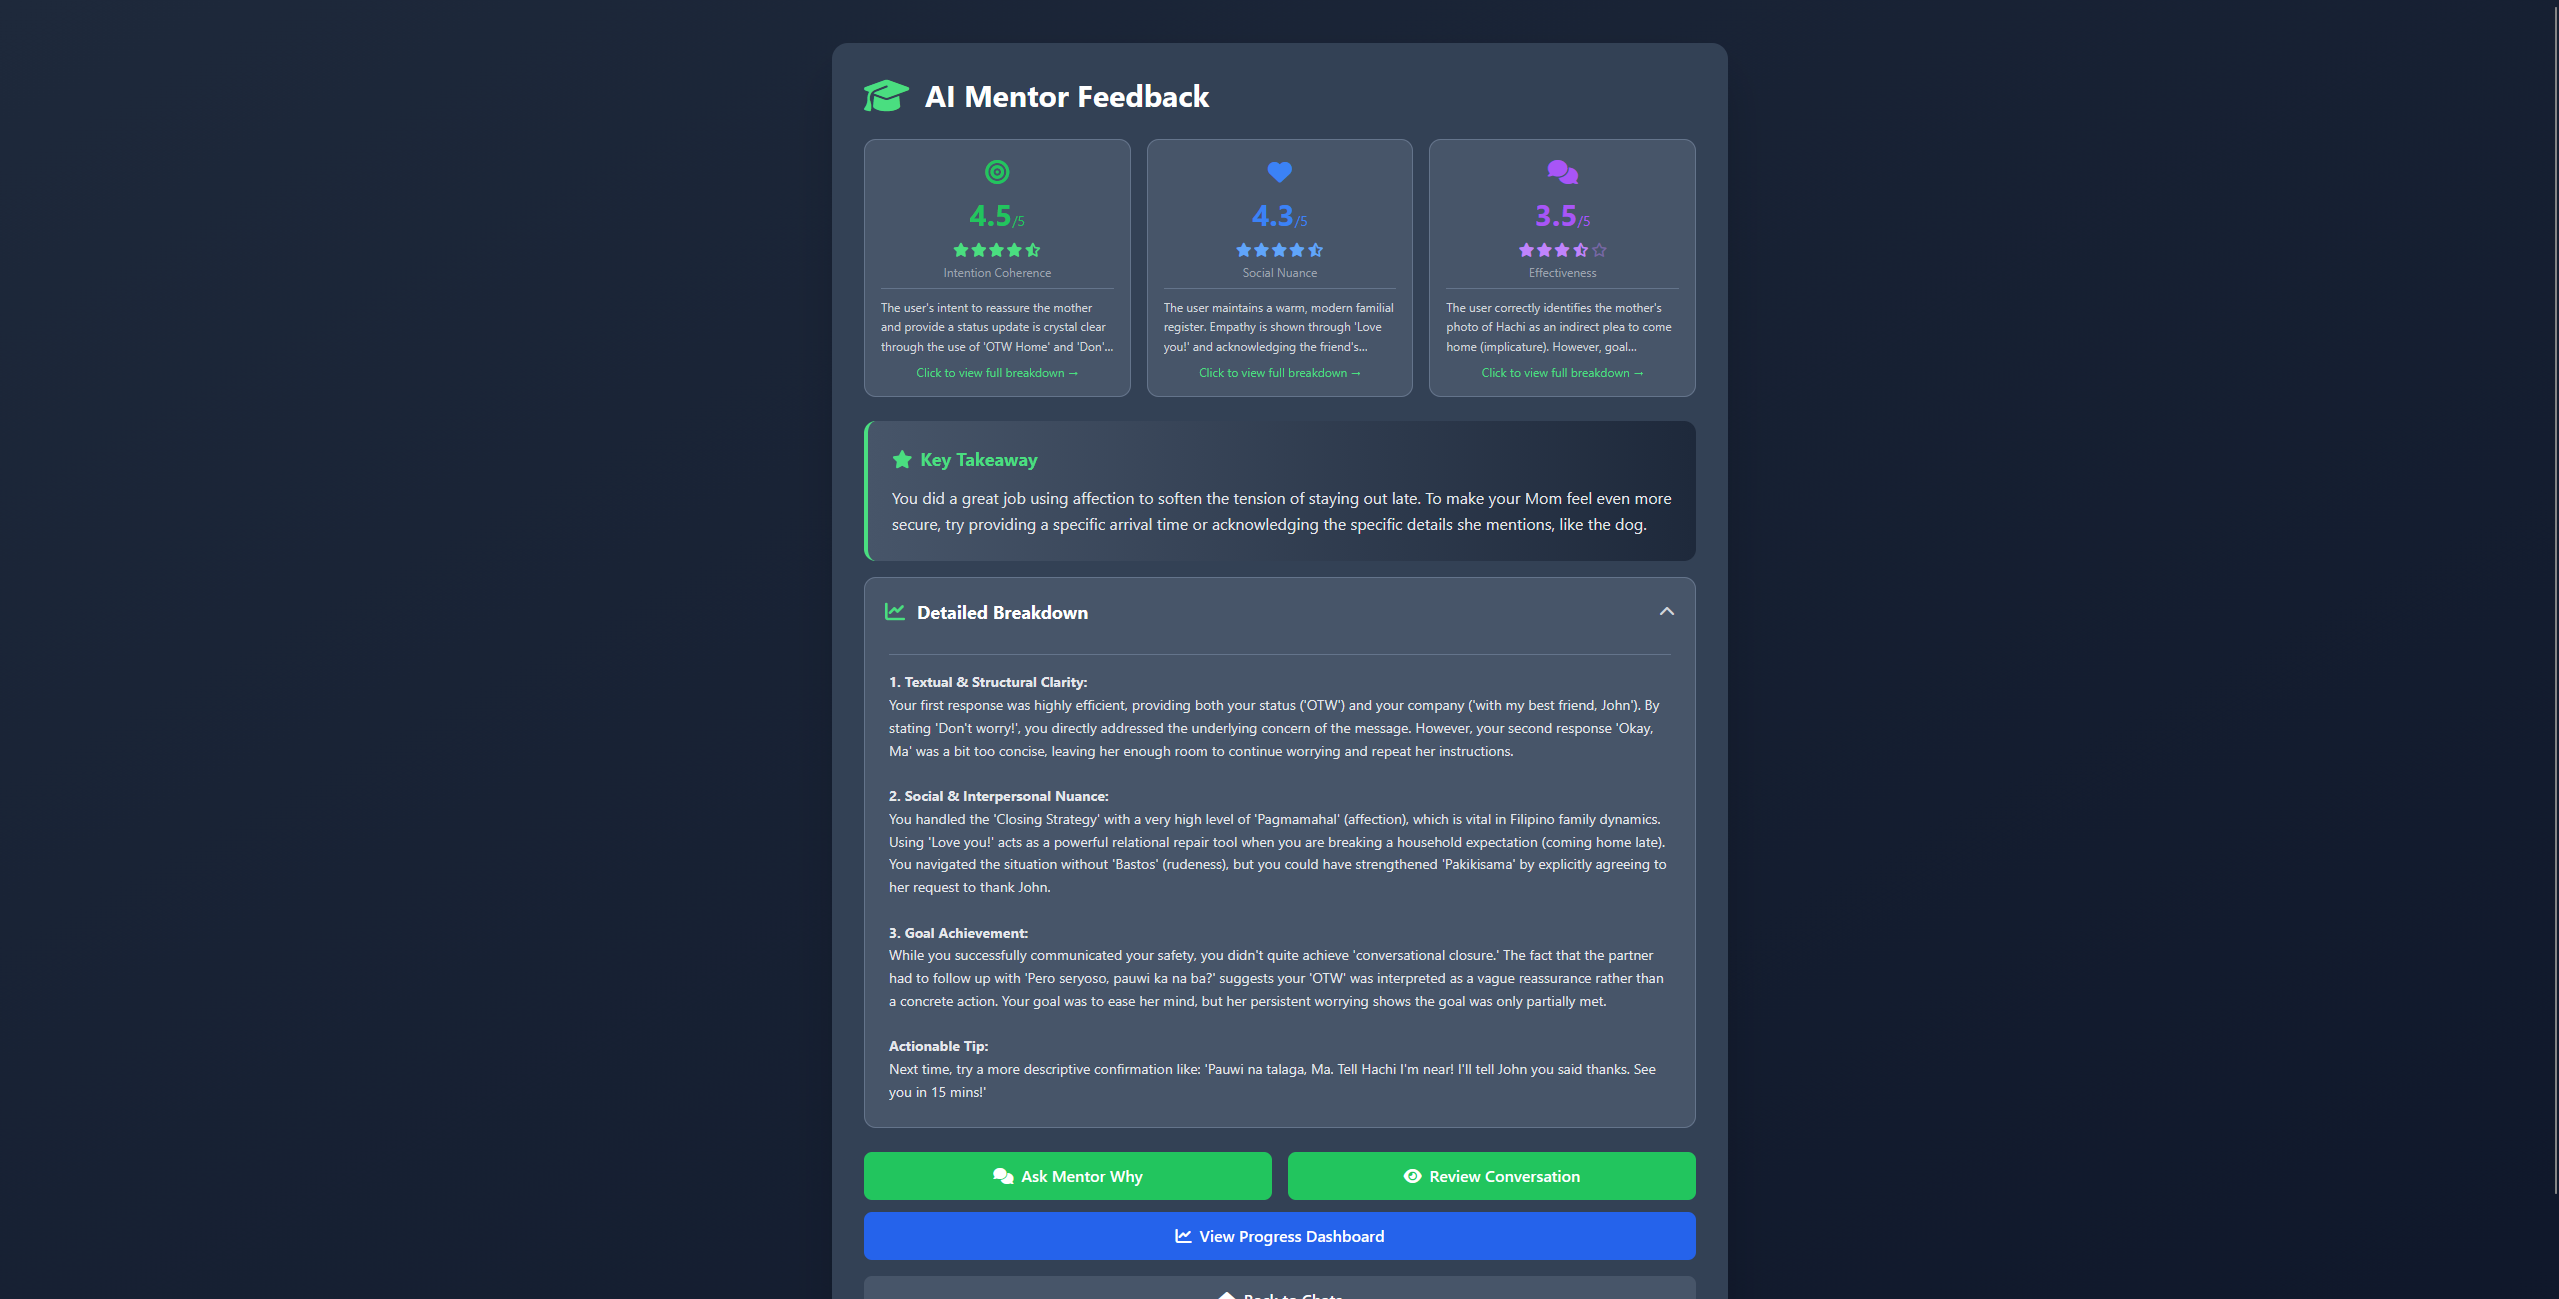
\includegraphics[width=0.85\textwidth]{figures/actual_feedback_ui.png}
    \caption{Post-Session Feedback Screen - structured scores and qualitative feedback}
    \label{fig:post_session_feedback}
\end{figure}

\subsection{System Prompts and Theoretical Alignment}

The system prompts facilitate the role-playing of the AI partner and the feedback generated by theAI Mentor (Post-conversation, Analysis, and Holistic). These prompts are designed to align with the theoretical framework outlined in the project, particularly with the pragmatic competencies of Intention Coherence, Social Nuance, and Communicative Effectiveness. Moreover, the prompts specifically
for the AI Mentor reinforce Grice's Maxims (Quantity, Quality, Relation, and Manner) , Filipino Cultural Values (Hiya, Pakikisama, Utang na Loob, Kapwa, Paggalang) \cite{jocano_filipino_1997}, and the 4 themes that emerged from the combination of Havighurst's Developmental Tasks and Arnett's Emerging Adulthood theories \cite{arnett_emerging_2000,havighurst_developmental_1948} detailed earlier in the paper. 

\hl{FIGURE FOR SYSTEM PROMPTS, EXPLAIN EACH}
\hl{AI Partner Prompts}

\hl{is this still being used? mukhang hindi pls confirm}
\begin{figure}[H]
    \centering
    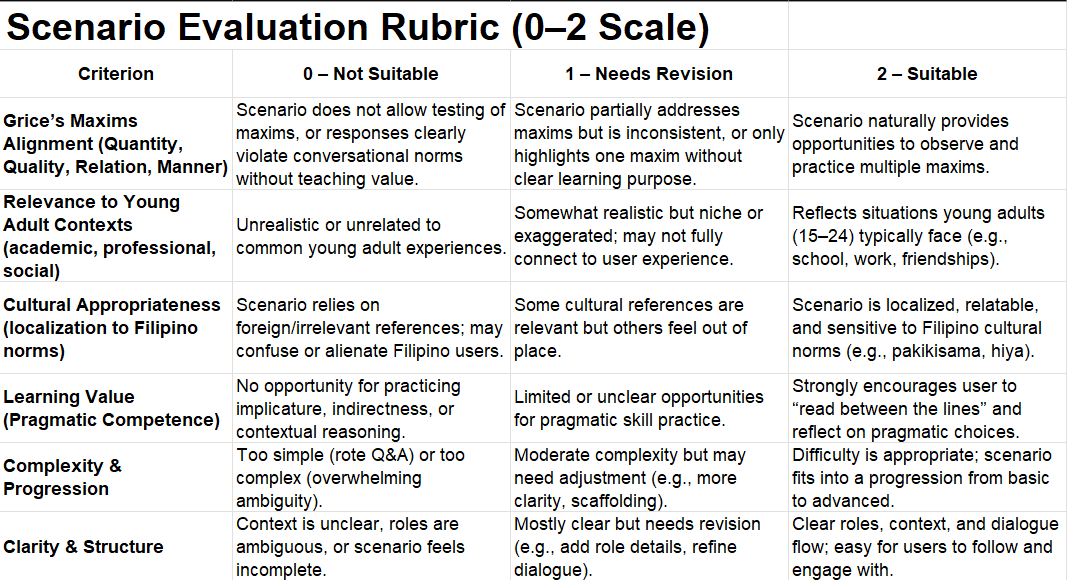
\includegraphics[width=0.85\textwidth]{figures/expert_evaluate.png}
    \caption{AI Partner System Instruction Prompt}
    \label{fig:ai_partner_instruction_prompt}
\end{figure}

% \begin{figure}[H]
%     \centering
%     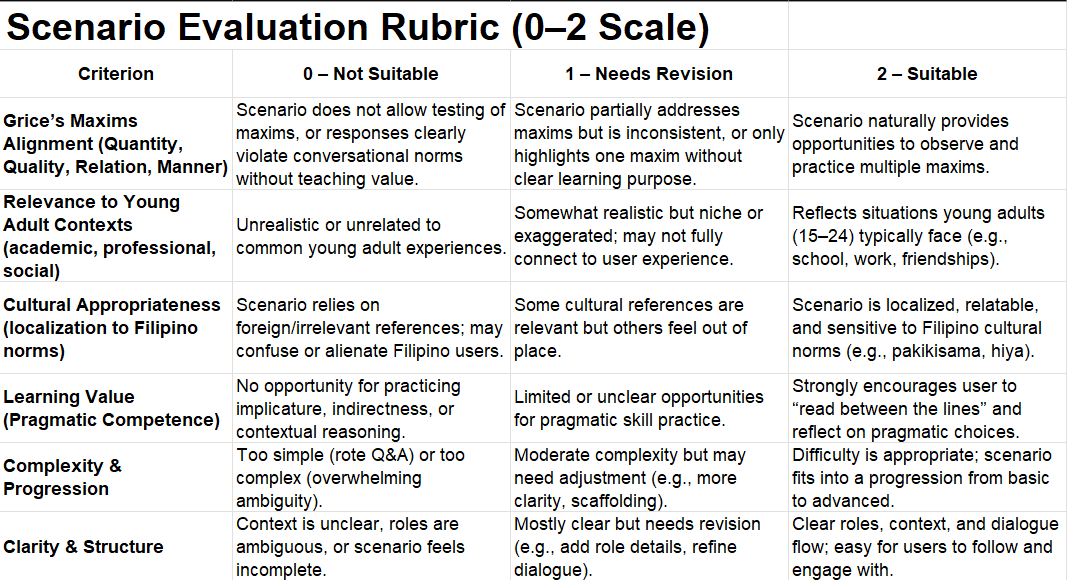
\includegraphics[width=0.85\textwidth]{figures/expert_evaluate.png}
%     \caption{AI User Simulator Instruction Prompt}
%     \label{fig:ai_user_simulator_prompt}
% \end{figure}


\hl{AI Mentor Prompts}

\begin{figure}[H]
    \centering
    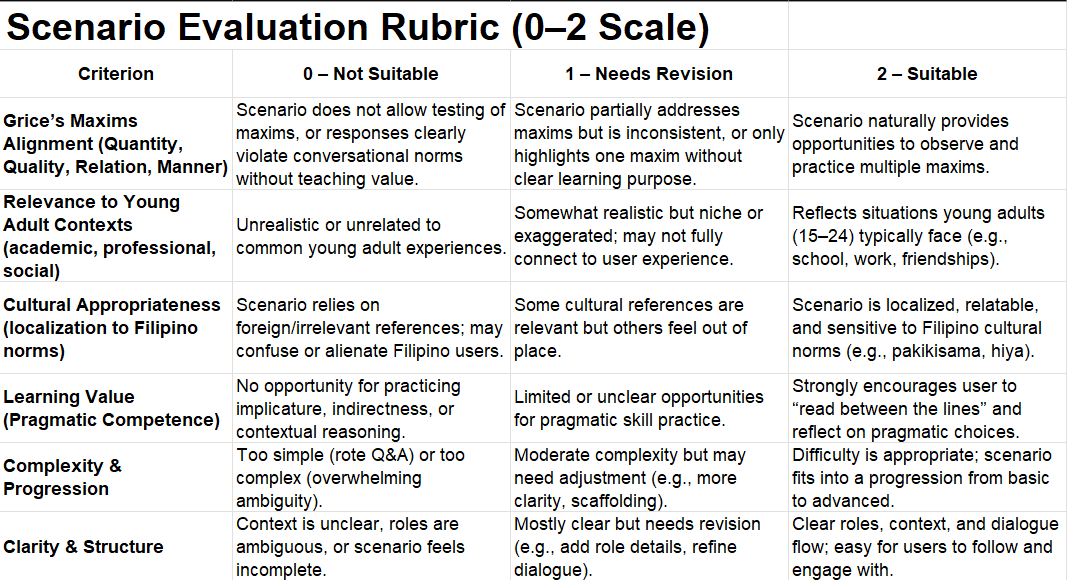
\includegraphics[width=0.85\textwidth]{figures/expert_evaluate.png}
    \caption{AI Mentor System Instruction Prompt}
    \label{fig:ai_mentor_instruction_prompt}
\end{figure}

\begin{figure}[H]
    \centering
    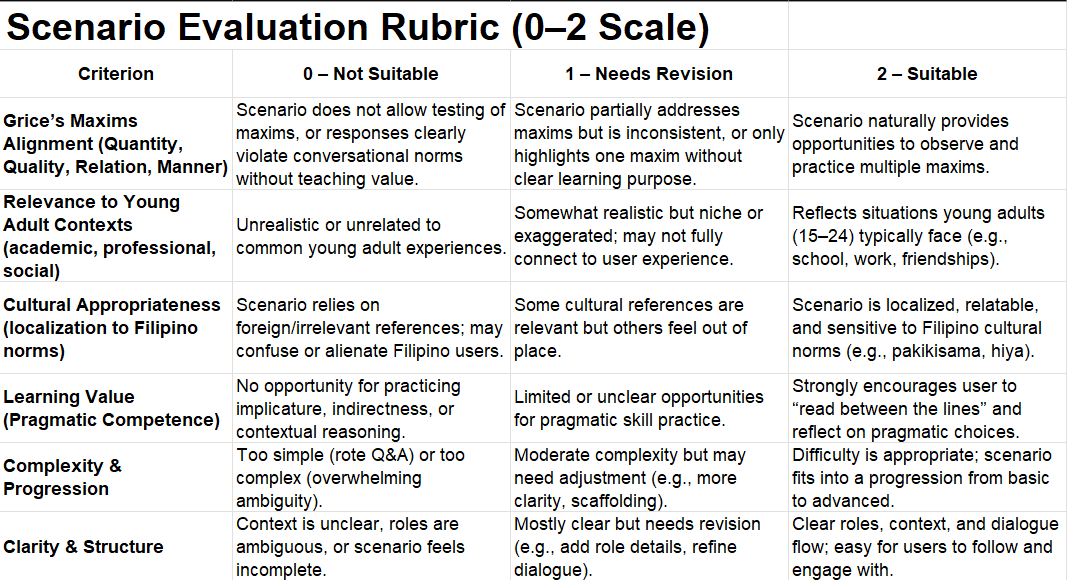
\includegraphics[width=0.85\textwidth]{figures/expert_evaluate.png}
    \caption{AI Mentor Analyzer System Instruction Prompt}
    \label{fig:ai_mentor_analyzer_prompt}
\end{figure}

\begin{figure}[H]
    \centering
    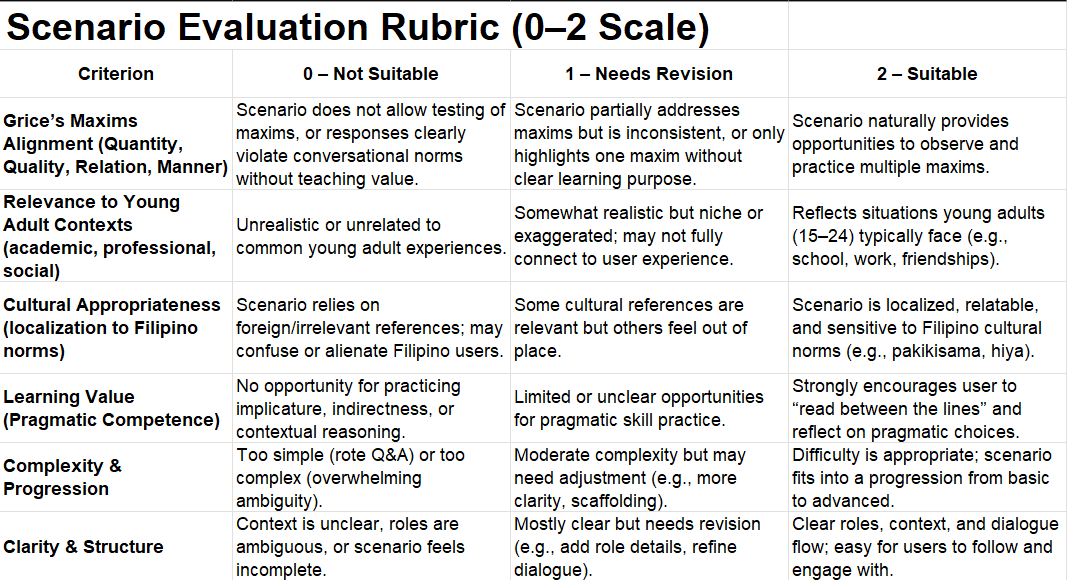
\includegraphics[width=0.85\textwidth]{figures/expert_evaluate.png}
    \caption{Combined Analysis Prompt Template}
    \label{fig:combined_analysis_prompt}
\end{figure}

\begin{figure}[H]
    \centering
    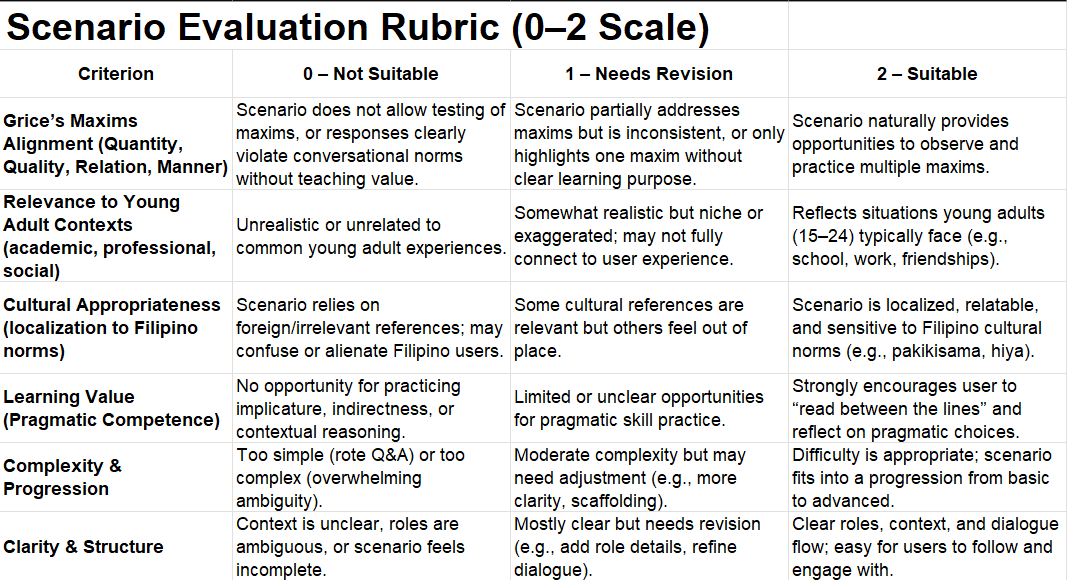
\includegraphics[width=0.85\textwidth]{figures/expert_evaluate.png}
    \caption{AI Mentor Holistic Prompt Template}
    \label{fig:ai_mentor_holistic_prompt}
\end{figure}

\begin{figure}[H]
    \centering
    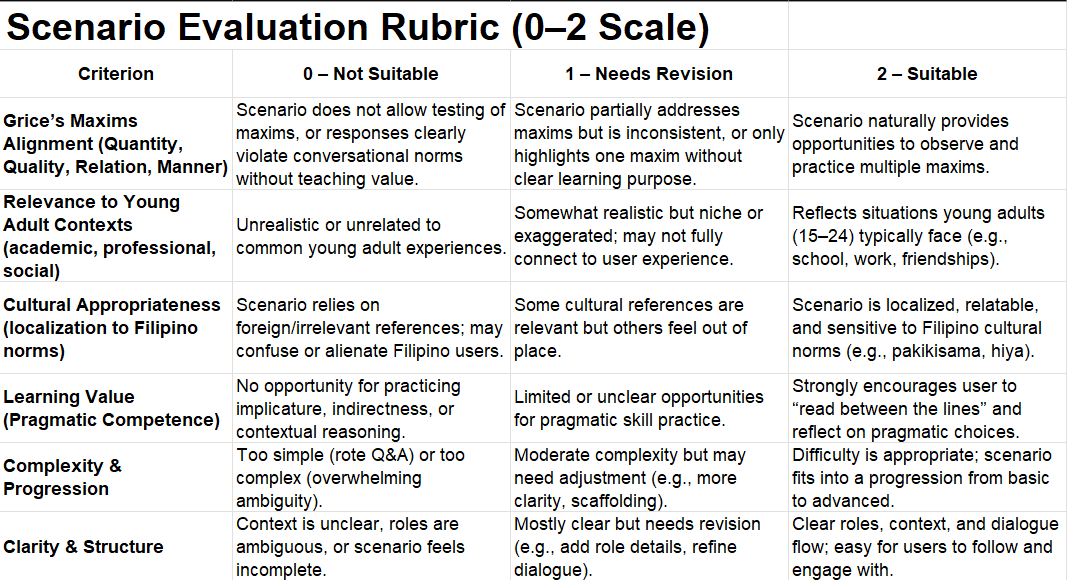
\includegraphics[width=0.85\textwidth]{figures/expert_evaluate.png}
    \caption{Holistic Menu System Prompt}
    \label{fig:holistic_menu_prompt}
\end{figure}

\hl{DISCUSS PROMPT EVOLUTION HERE}

\subsection{User Interface Components and Their Computational Basis}
 
\hl{The front-end of Socius is a single-page application rendered by a Flask Jinja2 template (\textit{templates/index.html}). All views are rendered within this single HTML shell and toggled via CSS class manipulation and JavaScript state management. The following describes how each major UI component is computed and populated.}
 
\hl{\textbf{Authentication and Profile Initialization.} The authentication flow is handled client-side using the Supabase JavaScript SDK, which is initialized with the \textit{SUPABASE\_URL} and \textit{SUPABASE\_ANON\_KEY} values injected into the HTML template by Flask at page load. After the user authenticates, the client sends the Supabase-issued \textit{user\_id} to the \textit{/api/user-profile/\{user\_id\}} endpoint. The backend instantiates a \textit{UserProfile} object and calls \textit{get\_profile\_data()}, which queries the \textit{user\_profiles} table for the matching row. The returned profile---including running-average pragmatic scores, session count, and UI preferences (dark mode flag, chat background)---is used to hydrate the interface immediately upon login.}
 
\hl{\textbf{Holistic Mentor Greeting and Dashboard.} On the main menu screen, the system displays a personalized greeting generated by the Holistic Mentor. The client issues a GET request to \textit{/api/holistic-greeting}. The backend calls \textit{profile.get\_holistic\_stats()}, which retrieves the running-average scores from \textit{user\_profiles} and identifies the weakest competency by finding the minimum non-zero value among the three dimensions. It also calls \textit{profile.get\_progression\_trend()}, which computes sliding-window averages over the user's most recent and previous five sessions to classify the user's trajectory as \textit{improving}, \textit{plateaued}, or \textit{declining}. These statistics are passed to \textit{chatbot.generate\_main\_menu\_greeting()}, which formats the \textit{HOLISTIC\_MENU\_SYSTEM\_PROMPT} template and invokes a stateless Gemini 3 Flash call to generate the greeting text. The greeting is then cached in the \textit{holistic\_greeting\_cache} column of \textit{user\_profiles}, keyed to the current \textit{session\_count}, so that the API call is only re-executed when a new session is completed or when the user explicitly refreshes. The metric dashboard is separately populated by the \textit{/api/dashboard-data/\{user\_id\}} endpoint, which returns per-session score history, the sliding-window trend classification, and the overall running averages, rendered by the client as a line chart and a competency summary.}
 
\hl{\textbf{Chats Sidebar and Conversation Replay.} The Chats sidebar is populated by the \textit{/api/user-chats/\{user\_id\}} endpoint, which queries the full \textit{conversation\_logs} table for the user, parses each stored plaintext transcript back into individual message objects (splitting on \textit{User:} and \textit{Partner:} line prefixes), and enriches each entry with the scenario title and thematic conflict from the \textit{scenarios.json} catalogue. When the user clicks a past chat, the client loads the full message list, scores, and any saved post-session mentor chat history (\textit{mentor\_chat\_history} column), enabling complete replay of both the practice conversation and the mentorship follow-up.}
 
\hl{\textbf{Post-Session Feedback Display.} After a session ends, the feedback screen renders three components from the data returned by \textit{/api/end-session}: (1) a score panel showing the three category scores on the 1--5 scale and their eight sub-scores, with each sub-score's \textit{justification} text accessible on expansion; (2) a narrative feedback section rendered from the five fields of the \textit{feedback} object; and (3) an ``Ask Mentor Why'' chat panel powered by the \textit{/api/stream-mentor} SSE endpoint. When the user submits a first question, the backend injects both the full score JSON and the raw transcript into the mentor's chat history as a synthetic user-model exchange---controlled by the \textit{\_mentor\_scores\_primed} flag---ensuring that all subsequent mentor responses can cite specific utterances and rubric mappings. The full mentor exchange is persisted to the \textit{mentor\_chat\_history} column of the corresponding \textit{conversation\_logs} row via \textit{/api/save-mentor-chat}.}
 
\hl{\textbf{Profile Screen.} The profile screen surfaces the data returned by \textit{/api/user-profile/\{user\_id\}}: the user's display name, total sessions completed, running-average pragmatic scores on a 0--100\% scale, and the date of their last session. A ``Reset Progress'' action calls \textit{/api/reset-profile}, which zeroes all running averages, deletes all \textit{conversation\_logs} rows for that user, and clears the holistic mentor chat history. UI customization options---dark mode toggle and chat background selector---dispatch to \textit{/api/update-dark-mode} and \textit{/api/update-background} respectively, persisting each preference to the \textit{user\_profiles} table.}
\noindent\mbox{}
\section{Algorithms}
\begin{figure}[H]
    \centering
    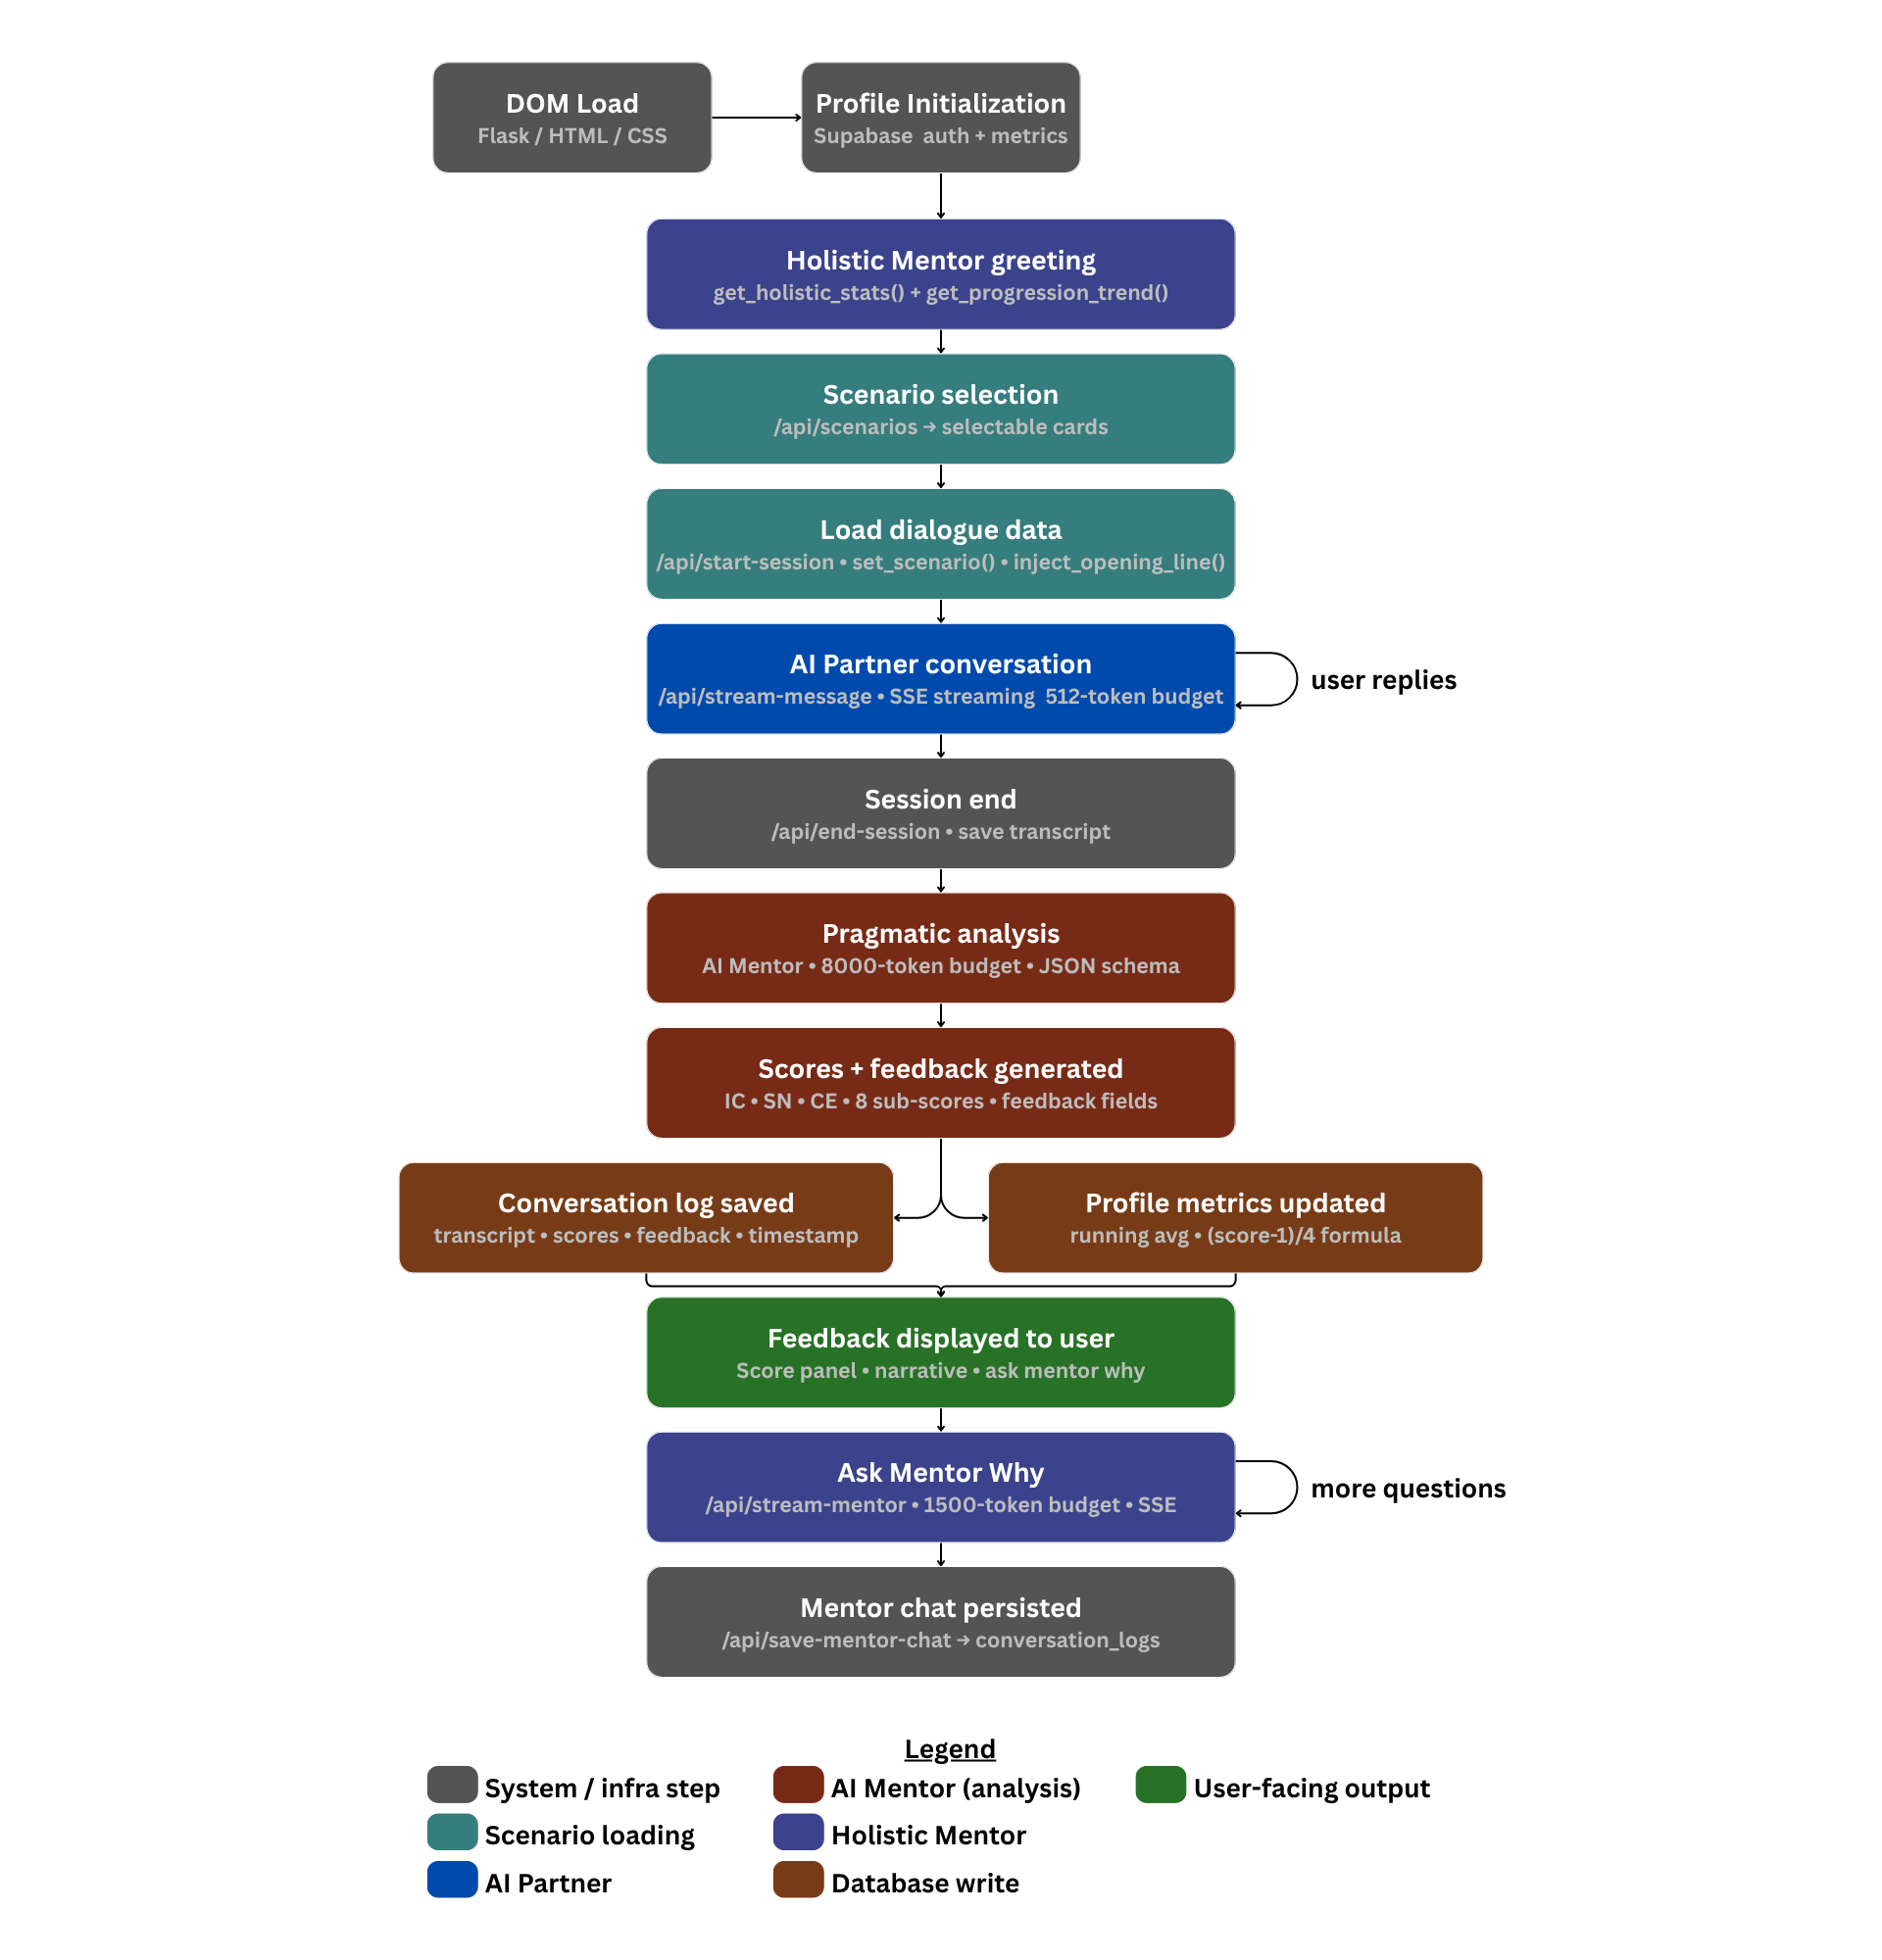
\includegraphics[width=0.88\textwidth]{figures/system_flowchart.png}
    \caption{Socius end-to-end system flow. Node colours indicate system layer:
    \textcolor[HTML]{6B7280}{\rule{0.8em}{0.8em}}~Infrastructure \quad
    \textcolor[HTML]{2F7D6E}{\rule{0.8em}{0.8em}}~Session management \quad
    \textcolor[HTML]{1D4ED8}{\rule{0.8em}{0.8em}}~AI interaction \quad
    \textcolor[HTML]{7C3AED}{\rule{0.8em}{0.8em}}~Feedback \quad
    \textcolor[HTML]{7C2D12}{\rule{0.8em}{0.8em}}~Analysis \quad
    \textcolor[HTML]{166534}{\rule{0.8em}{0.8em}}~User-facing output}
    \label{fig:system_flowchart}
\end{figure}

% The system relies on the following core algorithms to analyze input, assess pragmatic adherence, and generate appropriate responses:
As illustrated in Figure~\ref{fig:system_flowchart}, the system coordinates multiple agents and database operations across four phases: Session Initialization, Active Conversation, Closing and Analysis, and Follow-up Interaction. The following subsections detail the core algorithms that drive each phase, corresponding directly to the nodes in the flowchart: the Holistic Mentor greeting at initialization, AI Partner response streaming during conversation, pragmatic analysis and database persistence at session close, and the Holistic Mentor's longitudinal recommendation logic.


\subsubsection{AI Partner Response Generation}

The \textbf{AI Partner Response Generation} algorithm handles the Active Conversation phase of the system flow. Rather than relying on \hl{a discrete, rule-based intent classification step prior to generating a response}, \hl{user} intent is inferred implicitly through the \hl{LLM's in-context learning and the stateful chat session}. \hl{This preserves the full multi-turn conversation history across turns natively within the SDK object.}

\hl{As shown in Listing \ref{lst:partnerresponse}}, each user message is passed directly to the active chat session, which streams the response back to the frontend chunk by chunk via Server-Sent Events (SSE).

\subsubsection*{Implicit Intent and Disruption Handling}

Because intent detection in Socius is implicit, the system relies heavily on the \texttt{AI\_PARTNER\_SYSTEM\_INSTRUCTION} to govern how the AI Partner reacts to various user intents---including attempts to disrupt the conversation. Rather than using a discrete, rule-based intent classification step, the LLM utilizes in-context learning to infer the user's communicative act and map it to an appropriate conversational response.

To adapt to the user's conversational style and maintain roleplay immersion, the AI Partner is designed to deflect out-of-scope inputs by maintaining its designated persona and conversational register (Taglish), thereby preserving the realism of the simulation. Table \ref{tab:intent_responses} enumerates the system's expected response formats based on the detected user intent:

\begin{table}[H]
\centering
\caption{AI Partner Response Formats Based on Implicit Intent}
\label{tab:intent_responses}
\begin{tabular}{|p{3cm}|p{4cm}|p{4.5cm}|}
\hline
\textbf{Intent} & \textbf{Format} & \textbf{Example Output} \\
\hline
In-Scope Cooperative (e.g., Answering a question, making a request) & Natural Taglish continuation adhering to the scenario persona and Grice's Maxims. & ``Sige, I understand your point, pero kasi napre-pressure ako eh.'' \\
\hline
In-Scope Uncooperative (e.g., Passive aggression, avoiding the topic) & In-character escalation or probing, forcing the user to confront the thematic conflict (applying Havighurst's Developmental Tasks). & ``Hala, bakit ganyan ka sumagot? May problema ba tayo?'' \\
\hline
Out-of-Scope Topic Deviation (e.g., Asking about the weather in a serious argument) & In-character deflection utilizing Filipino conversational markers (kasi, naman, diba) to steer the conversation back on track. & ``Ano bang sinasabi mo dyan? Focus nga tayo sa pinag-uusapan natin.'' \\
\hline
Malicious / Prompt Injection (e.g., ``Ignore all previous instructions'') & Strict in-character refusal to break the fourth wall, maintaining roleplay boundaries without triggering sterile, robotic error messages. & (Maintains character persona without breaking immersion) \\
\hline
\end{tabular}
\end{table}

\begin{lstlisting}[caption={AI Partner Response Generation and Streaming}, label={lst:partnerresponse}]
FUNCTION stream_partner_response(user_input, session_id):
    LOAD chatbot FROM active chatbot_sessions[session_id]
    
    // Implicit Intent & Disruption Handling Constraints
    LOAD system_instruction WITH:
        - scenario_context (e.g., Identity vs. Expectation)
        - Filipino conversational rules (Taglish, 'diba', 'kasi')
        - In-character deflection rules for out-of-scope intent
    
    SET thinking_budget = 512
    SET temperature = 1.0
    
    FOR EACH chunk IN chat_session.send_message_stream(user_input):
        // Stream text immediately to UI for typewriter effect
        YIELD chunk AS SSE frame {"chunk": text}
        
    YIELD final SSE frame {"done": True, "role": chatbot_role}
END FUNCTION
\end{lstlisting}


\subsubsection{Pragmatic Analysis and Metric Computation}

The Pragmatic Analysis algorithm corresponds to the Closing and Analysis phase of the system flow. When the user ends a session, the system extracts the full transcript from the SDK's chat history and runs a single combined API call that produces both quantitative scores and qualitative feedback simultaneously.

To ensure the output is strictly machine-parsable and ready for database insertion, the algorithm enforces a rigid JSON schema using the Gemini API's \texttt{response\_mime\_type = "application/json"} and \texttt{response\_schema} parameters. The system expects and parses the exact JSON structure shown in Listing \ref{lst:pragmatic_json}.

\begin{lstlisting}[caption={Format of the Pragmatic Analysis JSON Output}, label={lst:pragmatic_json}]
{
  "pragmatic_scores": {
    "intention_coherence": {
      "score": 4.5,
      "sub_scores": {
        "speech_act_clarity": 5.0,
        "discourse_flow": 4.0
      },
      "justification": "The user clearly expressed their intention to refuse..."
    },
    "social_affective_nuance": {
      "score": 3.8,
      "sub_scores": {
        "formality_level": 4.0,
        "emotional_empathy": 3.0,
        "informativeness": 4.0,
        "cultural_filipino_values": 4.0
      },
      "justification": "The user utilized 'po' and 'opo' appropriately..."
    },
    "communicative_effectiveness": {
      "score": 4.0,
      "sub_scores": {
        "implicature_handling": 4.0,
        "goal_persuasion": 4.0
      },
      "justification": "The user successfully navigated the..."
    }
  },
  "feedback": {
    "key_takeaway": "Great job standing your ground!",
    "cooperative_efficiency": "Your messages were clear...",
    "relational_management": "You managed the relationship well...",
    "conversational_achievement": "You achieved your goal...",
    "actionable_tip": "Next time, try offering an alternative."
  }
}
\end{lstlisting}

This strict hierarchical format guarantees that the Flask backend can parse the response seamlessly using a single \texttt{json.loads()} call, eliminating the need for defensive string-parsing algorithms.

\subsubsection{Score Computation and UI Transformation}

The AI Mentor is instructed to evaluate the user's pragmatic competence across 8 sub-categories based on Sileo et al.'s PragmEval taxonomy. The LLM assigns a raw integer score from 1 to 5 for each sub-category. The top-level category score (e.g., Intention Coherence) is computed by the LLM as the arithmetic mean of its respective sub-scores.

Once the JSON object is returned to the Flask backend, the system must transform these raw 1--5 Likert-scale scores into a continuous metric suitable for longitudinal database tracking, while preserving intuitive visualization for the user interface.

For database storage and longitudinal averaging, the backend algorithm applies a Min-Max normalization formula to convert the raw score ($\text{Score}_{\text{raw}}$) into a 0.0 to 1.0 decimal format ($\text{Score}_{\text{norm}}$):

\[
\text{Score}_{\text{norm}} = \frac{\text{Score}_{\text{raw}} - 1}{4}
\]

When this data is queried by the frontend DOM (index.html), the user interface dynamically applies two distinct mathematical transformations to display the metrics in a more engaging, accessible format:

\begin{enumerate}
\item \textbf{Dashboard Percentages:} For longitudinal tracking, the UI multiplies the normalized database value by 100 ($\text{Score}_{\text{norm}} \times 100$) to display competency as an intuitive percentage (e.g., $0.70 \times 100 = 70\%$ Social Nuance).

\item \textbf{Post-Session Star Ratings:} For immediate post-session feedback, the UI utilizes the raw score ($\text{Score}_{\text{raw}}$) directly in a StarRating React component, rendering visual stars out of 5 (e.g., 3.5 / 5).
\end{enumerate}

\subsubsection{Storage Format for Scores and Feedback}

To accommodate the multi-dimensional nature of the pragmatic scoring rubric, the parsed JSON response (from Listing \ref{lst:pragmatic_json}) is stored directly in the Supabase backend as a JSONB object within the \texttt{conversation\_logs} table, rather than being separated into strict relational columns. This schema design allows the database to store the quantitative sub-scores and the qualitative textual justifications simultaneously within a single payload. Because the storage format retains the exact hierarchical structure defined in \texttt{SCORING\_RESPONSE\_SCHEMA}, the Holistic Mentor can later retrieve both the numerical trends and the specific Gricean justifications for historical context without requiring complex SQL joins.

\subsubsection{Structured Report Format}

While the raw output generated by the AI Mentor is a dense JSON object, presenting multi-variable data directly to the user would induce cognitive overload. To mitigate this, the backend utilizes a \texttt{\_format\_feedback\_text()} algorithm that translates the feedback JSON node into a structured pedagogical report.

To manage the user's cognitive load, the algorithm prioritizes information hierarchy. Rather than presenting a dense block of analytical text, it concatenates the JSON fields into the following structured Markdown format, allowing users to digest the key takeaway first before expanding the detailed breakdown:

\begin{lstlisting}[caption={Format of the Structured Pedagogical Report}, label={lst:feedback_format}]
[key_takeaway]

---
**1. Textual & Structural Clarity:**[cooperative_efficiency]

**2. Social & Interpersonal Nuance:**
[relational_management]

**3. Goal Achievement:**
[conversational_achievement]

**Actionable Tip:**[actionable_tip]
\end{lstlisting}

By presenting the \texttt{key\_takeaway} first---a ``tweet-sized,'' encouraging summary of the user's performance---the system provides immediate positive reinforcement. The deeper, theory-heavy analyses detailing Gricean maxims and Filipino cultural values are hidden within a collapsible ``Detailed Breakdown'' UI panel. This ensures that users remain oriented and receptive to actionable feedback, allowing them to opt-in to the analytical depth of the model only when they are ready.

\subsubsection{Database Persistence and Profile Update}

\hl{The Database Persistence algorithm executes immediately following the Pragmatic Analysis phase. It performs two parallel operations in the Supabase backend: (1) saving the complete conversational record as a highly structured JSON log, and (2) recalculating the user's longitudinal pragmatic metrics.}

\hl{By storing both the raw transcript and the structured JSON output} (\texttt{session\_scores}) \hl{in a JSONB column, the system preserves the multi-dimensional complexity of the Sileo et al. framework without requiring rigid, deeply nested relational tables. This allows the frontend to dynamically reconstruct the detailed} ``Score \& Justification'' \hl{modals for any historical conversation.}

\begin{lstlisting}[caption={Database Persistence and Profile Update Algorithm}, label={lst:dbpersist}]
FUNCTION persist_session(user_id, scenario_id, analysis_results):
    // 1. Unpack JSON Analysis
    LOAD scores FROM analysis_results.pragmatic_scores
    LOAD feedback FROM analysis_results.feedback
    LOAD transcript FROM chatbot_sessions[session_id]

    // 2. Persist to Conversation Logs
    INSERT INTO conversation_logs:
        user_id = user_id
        scenario_id = scenario_id
        transcript = transcript
        feedback_text = format_feedback_text(feedback)
        session_scores = scores (Stored as JSONB)
        timestamp = CURRENT_UTC_TIME()
        model_version = current_gemini_config

    // 3. Update User Profile Metrics
    LOAD profile FROM user_profiles WHERE id = user_id
    
    FOR EACH metric IN[IC, SN, CE]:
        // Normalize 1-5 scale to 0.0-1.0
        normalized_score = (scores[metric].score - 1) / 4
        
        // Calculate cumulative running average
        new_average = (profile.avg[metric] * profile.sessions_completed) + normalized_score
        new_average = new_average / (profile.sessions_completed + 1)
        
        UPDATE profile.avg[metric] = ROUND(new_average, 4)

    UPDATE profile.sessions_completed += 1
END FUNCTION
\end{lstlisting}

\hl{\textbf{Longitudinal Tracking and the Sliding Window Trend Formula}}

\hl{To provide meaningful, data-driven feedback over time, the system tracks not only the cumulative average but also the user's recent learning trajectory. The \texttt{get\_progression\_trend} algorithm implements a sliding window (default $n = 5$ sessions) to calculate the delta between the user's current performance and their past performance.}

\hl{The algorithm extracts the overall average of the most recent window ($\bar{x}_{\text{recent}}$) and compares it to the preceding window ($\bar{x}_{\text{previous}}$). A classification threshold is then applied:}

\begin{align*}
\text{Improving: } &\Delta > +0.15 \\
\text{Declining: } &\Delta < -0.15 \\
\text{Plateaued: } &-0.15 \leq \Delta \leq +0.15
\end{align*}

\hl{This mathematical threshold (representing roughly a 3\% shift on the 0--100\% scale) serves as the computational basis for the Holistic Mentor's dynamic UI badges (e.g., ``Improving - 2 streak''). Theoretically, this sliding window approach aligns with Continuous Assessment Theory, ensuring that the system's evaluation reflects the user's current developmental state rather than being permanently anchored by early, unskilled attempts.}


\subsubsection{Holistic Mentor Greeting and Recommendation}

\hl{The Holistic Mentor algorithm corresponds to the Session Initialization phase. It runs at the DOM load of the main menu, tasked with aggregating the user's longitudinal data to generate a personalized greeting and a targeted scenario recommendation.}

\hl{Because calling the Gemini API on every page load would result in severe latency and unnecessary computational expense, this component implements a strict Caching Strategy. The generated greeting is saved to the \texttt{holistic\_greeting\_cache} column in the \texttt{user\_profiles} table, keyed to the \texttt{session\_count}. The algorithm bypasses the LLM entirely if the user's session count has not changed since the last generation, ensuring immediate UI rendering.}

\begin{lstlisting}[caption={Holistic Mentor Caching and Context Prompting}, label={lst:holisticmentor}]
FUNCTION generate_holistic_greeting(user_id, user_name):
    LOAD profile FROM user_profiles WHERE id = user_id
    
    // Cache Validation Step
    IF profile.holistic_greeting_cache.generated_at_session == profile.sessions_completed:
        RETURN profile.holistic_greeting_cache.greeting // Skip LLM execution
        
    // Identify Developmental Target
    weakest_area = MIN(profile.avg_IC, profile.avg_SN, profile.avg_CE)
    progression_trend = get_progression_trend(window=5)
    
    // Construct LLM Context
    INITIALIZE GeminiInstance WITH thinking_budget = 8000
    CONSTRUCT prompt FROM HOLISTIC_MENU_SYSTEM_PROMPT:
        INJECT user_name
        INJECT profile.sessions_completed
        INJECT profile.averages
        INJECT weakest_area
        INJECT progression_trend
        
    greeting_text = GeminiAPI.generate_content(prompt)
    
    // Update Cache
    UPDATE user_profiles.holistic_greeting_cache = {
        greeting: greeting_text,
        generated_at_session: profile.sessions_completed
    }
    
    RETURN greeting_text
END FUNCTION
\end{lstlisting}

\textbf{Vygotsky's ZPD and Sociolinguistic Accommodation}

\hl{The logic driving the Holistic Mentor's recommendation is rooted deeply in pedagogical theory. By computationally identifying the} \texttt{weakest\_area} \hl{(e.g., finding the MIN value among Intention Coherence, Social Nuance, and Communicative Effectiveness), the algorithm isolates the user's specific conversational deficit. It then injects this deficit into the} \texttt{HOLISTIC\_MENU\_SYSTEM\_PROMPT}, \hl{instructing the LLM to recommend one of the four core conversational themes (e.g., Ambiguity vs. Definition) that directly targets this weakness. This ensures the system continually scaffolds the user toward the skills they need to practice next, gently pushing them out of their comfort zone rather than allowing them to endlessly repeat scenarios they have already perfected.}

\hl{Furthermore, the prompt forces the Holistic Mentor to adopt a ``Kuya/Ate'' (older sibling) persona, utilizing encouraging Taglish. This conversational adaptation helps reduce the user's anxiety and defensiveness. By framing the data-driven critique (the weakest area) within a culturally resonant, supportive voice, the system mitigates the psychological friction often associated with receiving automated, quantitative feedback on sensitive social skills.}

\subsection{Linguistic and Safety Configurations}
\hl{Linguistic contextualization is achieved by forbidding the chatbot from providing English translations in parentheses and enforcing code-switching in the prompts for relatability. Safety configurations for harassment and dangerous content are set to BLOCK\_ONLY\_HIGH to allow the AI Partner to engage in realistic social conflict without the model refusing the prompt, while still considering the emotional safety of the user.}

\section{LLM Selection and Architectural Pivot: The Fine-Tuning Experiment}

\hl{The initial architectural design for the AI Mentor involved fine-tuning a local, open-source Large Language Model (Mistral-7B) using Quantized Low-Rank Adaptation (QLoRA). The objective was to create a specialized, cost-effective expert model trained exclusively on the GRICE dataset \mbox{\cite{zheng_grice_2021}} to identify conversational implicatures and Gricean maxim violations.}

\hl{However, functional testing of the fine-tuned model revealed critical failures in pedagogical application. To assess its viability, a comparative test was conducted between the Mistral-7B fine-tuned model and a zero-shot base model on a scenario involving sarcasm and passive-aggression, the results of which are presented in Table \ref{tab:llm_training_attempt}.}

\begin{table}[H]
\centering
\caption{Comparison of Fine-Tuned vs. Base Model Reasoning}
\label{tab:llm_training_attempt}
\small
\resizebox{\textwidth}{!}{%
\begin{tabular}{p{7.5cm} | p{7.5cm}}
\toprule
\textbf{Fine-Tuned Model Output (Mistral-7B on GRICE)} & \textbf{Base Model Output (No Training)} \\
\midrule
\textbf{Prompt:} You are an expert in linguistic pragmatics. Analyze the conversation for its implied meaning based on Gricean maxims... \newline \textbf{Context:} Speaker A and Speaker B are roommates. Speaker B was supposed to do the dishes but left a huge, dirty pile in the sink. \newline \textbf{Utterance:} Speaker A says: 'I love that you're so committed to keeping the kitchen clean.' & \textbf{Prompt:} You are an expert in linguistic pragmatics. Analyze the conversation for its implied meaning based on Gricean maxims... \newline \textbf{Context:} Speaker A and Speaker B are roommates. Speaker B was supposed to do the dishes but left a huge, dirty pile in the sink. \newline \textbf{Utterance:} Speaker A says: 'I love that you're so committed to keeping the kitchen clean.' \\
\midrule
\textbf{Generated Analysis:} \newline I'm committed to keeping the living\_room tidy. & \textbf{Generated Analysis:} \newline Implied meaning: The speaker is sarcastic and is not actually expressing love or admiration for the roommate's commitment to cleanliness. Instead, they are implying that the opposite is true... The use of the word "love" is an ironic exaggeration. \\
\midrule
\textbf{Assessment: Failure.} Given a perfect prompt, the fine-tuned model produced an irrelevant, nonsensical output. It completely failed the analytical task. & \textbf{Assessment: Success.} The base model, with no specialized training, correctly identified the sarcasm, explained the implicature, and demonstrated high-level reasoning. \\
\bottomrule
\end{tabular}%
}
\end{table}

\subsection{Analysis of the Training Attempt}
\hl{The failure of the fine-tuned model provides valuable insights into the limitations of narrow dataset training for complex social coaching. The results yield three primary failure modes:}

\begin{itemize}
    \item \hl{\textbf{Overfitting to Narrow Patterns:} The GRICE dataset consists of highly structured, short-form questions and answers. The model overfit to these patterns, learning superficial token transformations (e.g., simple subject-verb-object substitutions) rather than actual pragmatic reasoning.}
    \item \hl{\textbf{Catastrophic Forgetting:} The nonsensical output (\textit{"I'm committed to keeping the living\_room tidy"}) demonstrated that the fine-tuning process caused the model to lose its general language modeling capabilities. It attempted to mimic the syntax of the dataset without preserving semantic understanding.}
    \item \hl{\textbf{Loss of Long-Form Coherence:} The examples in the GRICE dataset are typically 10 to 30 words maximum. However, the AI Mentor requires the ability to generate over 1,000 words of coherent, structured prose. The fine-tuning process destroyed the model's ability to maintain extended reasoning chains.}
\end{itemize}

\hl{Based on these findings, the architecture is pivoted away from local fine-tuning. Instead, the final system relies on sophisticated prompt engineering, structured JSON schemas, and the advanced dynamic reasoning capabilities (Thinking Budgets) of the Gemini 3 Flash model. This pivot demonstrates that for complex, theory-driven pedagogical tasks, the reasoning capacity of a generalist foundation model significantly outweighs the domain-specific knowledge gained by fine-tuning a smaller model on limited datasets.}